\subsection{Class Diagram}

The class diagram shown in Figure~\ref{fig:class-diagram} provides an overview of the
main components of the system and their relationships.

The architecture is structured into the following layers:

\begin{itemize}
    \item \textbf{Controller Layer} -- implemented through Java Servlets, responsible for handling HTTP requests and responses. Examples include \texttt{UploadNoteServlet}, \texttt{LoginServlet}, and \texttt{SearchNoteServlet}.

    \item \textbf{Model Layer} -- composed of Plain Java Objects representing the core entities of the application, such as \texttt{User}, \texttt{Note}, \texttt{Course}, \texttt{Favorite}, and \texttt{Rating}.

    \item \textbf{DAO Layer} -- responsible for data persistence and retrieval through JDBC interaction with the PostgreSQL database. Examples include \texttt{NoteDAO}, \texttt{UserDAO}, and \texttt{RatingDAO}.

    \item \textbf{Utility / Service Layer} -- provides supporting functionalities such as database connection management and file storage. In particular, \texttt{DBConnection} handles database connectivity, while \texttt{StorageService} manages file upload and retrieval from cloud storage.
\end{itemize}

This layered design promotes loose coupling between components and simplifies future
extensions of the system.

\begin{figure}[H]
    \centering
    \fbox{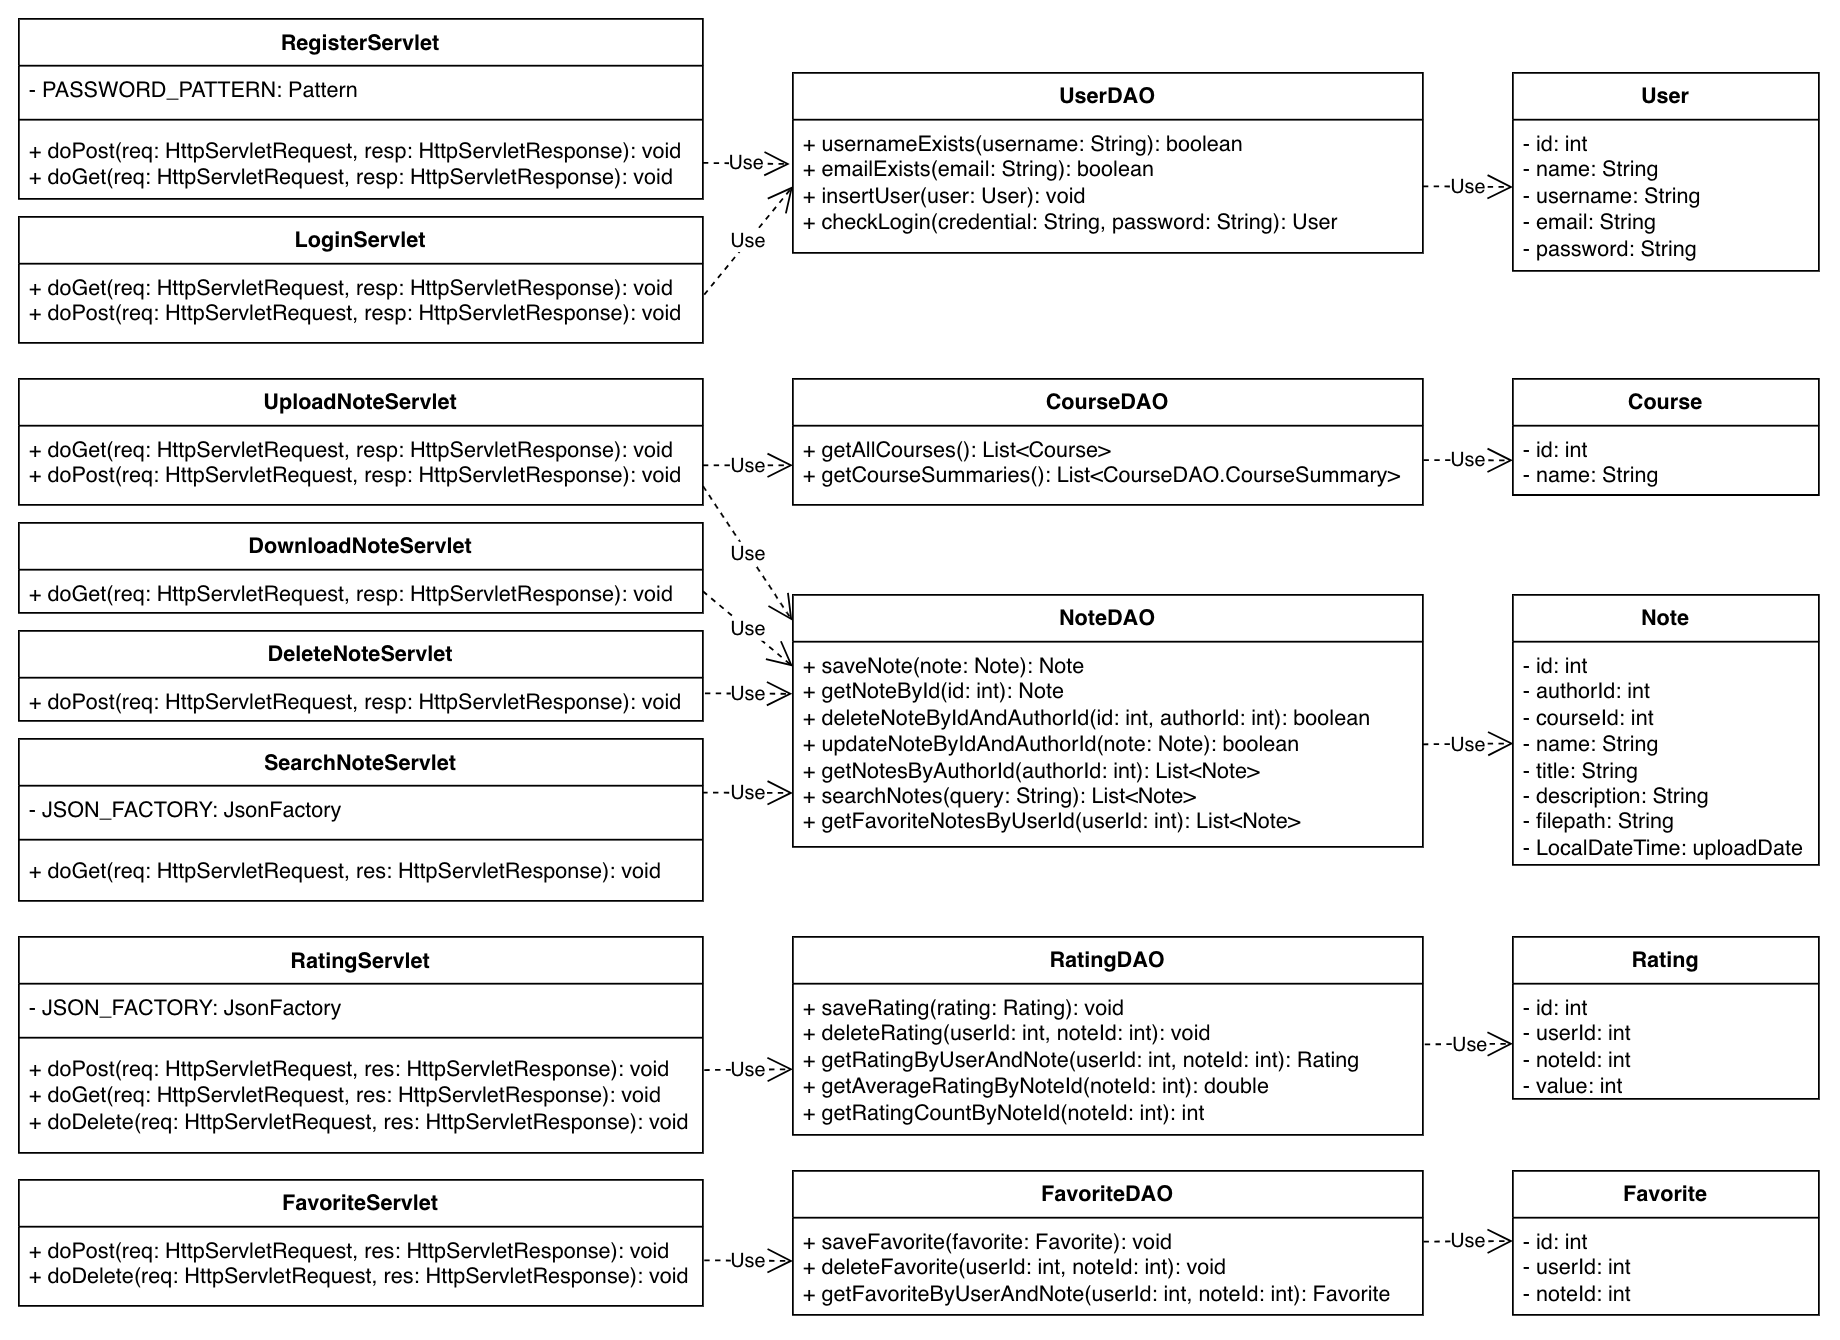
\includegraphics[width=0.95\textwidth]{../diagrams/classDiagram.png}}
    \caption{Class Diagram of the Lecture Notes App}
    \label{fig:class-diagram}
\end{figure}